\documentclass[10pt,letterpaper]{article}
\usepackage{amssymb} %maths
\usepackage{amsmath} %maths
\usepackage{polynom}
\usepackage{graphicx}
\usepackage{pgfplots}
\usepackage{tikz}
\usepackage{caption}
\usepackage{subcaption}
\usepackage[margin=0.5in]{geometry}
\usepackage{multicol}
\usepackage{mhchem}
\usepackage{enumitem}
\usepackage{mdframed}
\usetikzlibrary{arrows.meta,angles,quotes}
\pagenumbering{gobble}

\newenvironment{defbox}[2]
    {\mdfsetup{frametitle={
        \tikz[baseline=(current bounding box.east),outer sep=0pt]
        \node[anchor=east,rectangle,fill=#2!20]
        {\strut #1};}}
    \mdfsetup{innertopmargin=10pt,innerbottommargin=10pt, backgroundcolor=#2!2, linecolor=#2!20,%
linewidth=2pt,topline=true,
frametitleaboveskip=\dimexpr-\ht\strutbox\relax,}
\begin{mdframed}[]\relax
    }
    {
        \end{mdframed}
    }

\begin{document}
\begin{center}
    \Large\textbf{AP Chemistry Thermodynamics Handout}
\end{center}
\begin{multicols*}{2}
    \begin{defbox}{Important Terms}{blue}
        \begin{itemize}
            \item \textbf{Enthalpy ($\Delta H$):} Heat content of a system at constant pressure.
            \item \textbf{Entropy ($\Delta S$):} Measure of disorder or randomness in a system.
            \item \textbf{Gibbs Free Energy ($\Delta G$):} Energy available to do work; determines spontaneity.
            \item \textbf{Exothermic:} Releases heat; \textcolor{red}{$\Delta H < 0$}.
            \item \textbf{Endothermic:} Absorbs heat; \textcolor{blue}{$\Delta H > 0$}.
            \item \textbf{Spontaneous:} Occurs without external input; \textcolor{green!50!black}{$\Delta G < 0$}.
            \item \textbf{Heat Transfer:} Energy transfers from \textcolor{red}{hot} to \textcolor{blue}{cold} objects until they are equal.
            \item \textbf{Calorimetry:} The science of measuring heat transfer.
        \end{itemize}
    \end{defbox}
    \begin{defbox}{Equations}{red}
        \textbf{Energy}
        \begin{itemize}
            \item Heat transfer: $\Delta H = m \cdot c \cdot \Delta T$ 
            \item Phase change: $\Delta H = m \cdot H_{\text{fus/vap}}$
            \item Power: $P = \frac{W}{\Delta t}$
            \item Gibbs free energy: $\Delta G = \Delta H - T \cdot \Delta S$
            \item Work: $W = F \cdot s$
            \item Force: $F = m \cdot a$
        \end{itemize}
        \textbf{Waves\footnote{For these equations use units of meters, seconds, joules, and kilograms.}}
        \begin{itemize}
            \item Wave: $c = \lambda \cdot \nu$ ($c=3.00 \times 10^8 \text{ m/s}$)
            \item Planck: $E = h \cdot \nu$ ($h=6.626 \times 10^{-34} \text{ J·s}$)
            \item Einstein: $E = mc^2$
        \end{itemize}
    \end{defbox}
    \begin{defbox}{Laws of Thermodynamics}{green!70!blue}
        \begin{enumerate}
            \item \textbf{Conservation of energy:} Energy cannot be created or destroyed, only transformed.
            \item \textbf{Entropy:} The total entropy of an isolated system increases over time. Disorder increases.
            \item \textbf{Max Efficiency:} Efficiency approaches 100\% as temperature approaches absolute zero. 
        \end{enumerate}
    \end{defbox}
    \begin{defbox}{Energy Types}{purple}
    \textbf{Kinetic Energy (Movement)}
    \begin{itemize}
        \item Mechanical
        \item Electrical
        \item Thermal
        \item Light
        \item Sound
        \item Wind
    \end{itemize}
    \textbf{Potential Energy (Stored)}
    \begin{itemize}
        \item Chemical
        \item Gravitational
        \item Nuclear
    \end{itemize}
    \end{defbox}
    \begin{defbox}{System Types}{orange}
        \begin{itemize}
            \item \textbf{Open System:} Can exchange both energy and matter with its surroundings.
            \item \textbf{Closed System:} Can exchange energy but not matter with its surroundings.
            \item \textbf{Isolated System:} Cannot exchange energy or matter with its surroundings.
        \end{itemize}
    \end{defbox}
    \begin{defbox}{Water Phase Change Constants}{cyan}
        \begin{itemize}
            \item \textbf{Heat of Fusion ($H_{\text{fus}}$):} $334 \text{ J/g}$
            \item \textbf{Heat of Vaporization ($H_{\text{vap}}$):} $2260 \text{ J/g}$
            \item \textbf{Specific Heat Capacity (l) ($c_l$):} $4.184 \text{ J/g·°C}$
            \item \textbf{Specific Heat Capacity (s) ($c_s$):} $2.05 \text{ J/g·°C}$
            \item \textbf{Specific Heat Capacity (g) ($c_g$):} $1.996 \text{ J/g·°C}$
        \end{itemize}
    \end{defbox}
    \begin{defbox}{Spontaneity Table}{teal}
        \begin{center}
            \begin{tabular}{c|c|c}
                \textbf{$\Delta H$} & \textbf{$\Delta S$} & \textbf{Spontaneity} \\
                \hline
                $-$ & $+$ & Always spontaneous \\
                $-$ & $-$ & Spontaneous at low T \\
                $+$ & $+$ & Spontaneous at high T \\
                $+$ & $-$ & Never spontaneous \\
            \end{tabular}
        \end{center}
    \end{defbox}
    \begin{defbox}{Gibbs and Equilibrium}{magenta}
        The quantity of Gibbs free energy is related to the equilibrium constant ($K$) by the equation:
        \begin{equation*}
            \Delta G = -RT \ln K
        \end{equation*}  
    \end{defbox}
    \begin{defbox}{Hess's Law}{yellow!80!black}
        The total enthalpy change for a reaction is the same, regardless of the pathway taken. 
        \begin{itemize}
            \item $\Delta H_{\text{overall}} = \sum \Delta H_{\text{steps}}$
            \item Use this to calculate enthalpy changes for reactions that are difficult to measure directly.
        \end{itemize}
        For example if for the following reactions:
        \begin{align*}
            \ce{2C(s) + O2(g) &-> 2CO(g)} \quad \Delta H_1 = -221.0 \text{ kJ/mol} \\
            \ce{2CO(g) + O2(g) &-> 2CO2(g)} \quad \Delta H_2 = -283.0 \text{ kJ/mol}
        \end{align*}
        Then the enthalpy change for the reaction $\ce{2C(s) + 2O2(g) -> 2CO2(g)}$ can be calculated as:
        \begin{align*}
            \Delta H_{\text{overall}} &= \Delta H_1 + \Delta H_2 \\
            &= -221.0 \text{ kJ/mol} + (-283.0 \text{ kJ/mol}) \\
            &= -504.0 \text{ kJ/mol}
        \end{align*}
    \end{defbox}
    \begin{defbox}{Energy Diagrams}{brown}
        \begin{center}
            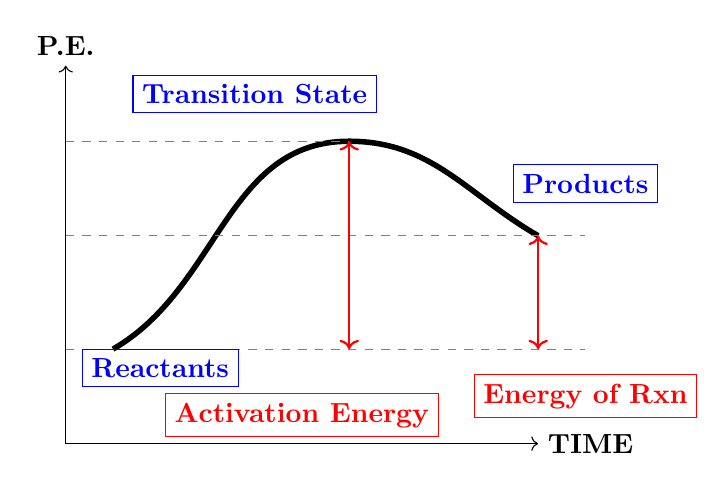
\begin{tikzpicture}[scale=1.2]
                % Axes
                \draw[->] (0,0) -- (5,0) node[right] {\textbf{TIME}};
                \draw[->] (0,0) -- (0,4) node[above] {\textbf{P.E.}};
                
                % Energy curve for endothermic reaction
                \draw[thick, black, line width=2pt] (0.5,1) to[out=30,in=180] (3,3.2) to[out=0,in=150] (5,2.2);
                
                % Dashed lines for energy levels
                \draw[dashed, gray] (0,1) -- (5.5,1);
                \draw[dashed, gray] (0,2.2) -- (5.5,2.2);
                \draw[dashed, gray] (0,3.2) -- (3,3.2);
                
                % Labels in boxes
                \node[draw, blue] at (1,0.8) {\textbf{Reactants}};
                \node[draw, blue] at (5.5,2.75) {\textbf{Products}};
                \node[draw, blue] at (2,3.7) {\textbf{Transition State}};
                
                % Energy labels in red boxes
                \node[draw, red] at (2.5,0.3) {\textbf{Activation Energy}};
                \node[draw, red] at (5.5,0.5) {\textbf{Energy of Rxn}};
                
                % Arrows showing energy differences
                \draw[<->, thick, red] (3,1) -- (3,3.2);
                
                % Arrow from transition state to activation energy label
                \draw[<->, thick, red] (5,1) -- (5,2.2);
            \end{tikzpicture}
        \end{center}
        \textbf{Key Features:}
        \begin{itemize}
            \item \textbf{Activation Energy:} Energy barrier that must be overcome for reaction to proceed.
            \item \textbf{Transition State:} Highest energy point along the reaction pathway.
            \item \textbf{Energy of Reaction:} Overall energy change from reactants to products.
        \end{itemize}
    \end{defbox}
    \begin{defbox}{Catalysts}{gray}
        \textbf{Definition:} Substances that increase the rate of a chemical reaction without being consumed in the process. They work by lowering the activation energy of a reaction, allowing it to proceed more quickly.
        \begin{itemize}
            \item \textbf{Enzymes:} Biological catalysts that speed up reactions in living organisms.
            \item \textbf{Heterogeneous Catalysts:} Catalysts that are in a different phase than the reactants (e.g., solid catalyst with gas reactants).
            \item \textbf{Homogeneous Catalysts:} Catalysts that are in the same phase as the reactants (e.g., acid catalyst in a liquid reaction).
        \end{itemize}
    \end{defbox}
    \begin{defbox}{Energy Bar Diagrams}{orange}
        \begin{center}
            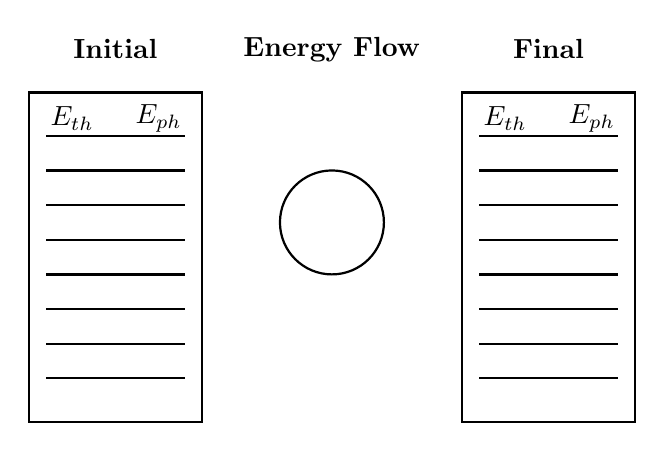
\begin{tikzpicture}[scale=1.1]
                % Section labels
                \node at (1.5,4.5) {\textbf{Initial}};
                \node at (4,4.5) {\textbf{Energy Flow}};
                \node at (6.5,4.5) {\textbf{Final}};
                
                % Initial section - left side
                \draw[thick] (0.5,4) rectangle (2.5,0.2);
                
                % Energy levels - Initial (left)
                \draw[thick] (0.7,3.5) -- (2.3,3.5);
                \draw[thick] (0.7,3.1) -- (2.3,3.1);
                \draw[thick] (0.7,2.7) -- (2.3,2.7);
                \draw[thick] (0.7,2.3) -- (2.3,2.3);
                \draw[thick] (0.7,1.9) -- (2.3,1.9);
                \draw[thick] (0.7,1.5) -- (2.3,1.5);
                \draw[thick] (0.7,1.1) -- (2.3,1.1);
                \draw[thick] (0.7,0.7) -- (2.3,0.7);
                
                % Labels for Initial
                \node at (1,3.7) {$E_{th}$};
                \node at (2,3.7) {$E_{ph}$};
                
                
                % Energy Flow circle
                \draw[thick] (4,2.5) circle (0.6);
                
                % Final section - right side  
                \draw[thick] (5.5,4) rectangle (7.5,0.2);
                
                % Energy levels - Final (right)
                \draw[thick] (5.7,3.5) -- (7.3,3.5);
                \draw[thick] (5.7,3.1) -- (7.3,3.1);
                \draw[thick] (5.7,2.7) -- (7.3,2.7);
                \draw[thick] (5.7,2.3) -- (7.3,2.3);
                \draw[thick] (5.7,1.9) -- (7.3,1.9);
                \draw[thick] (5.7,1.5) -- (7.3,1.5);
                \draw[thick] (5.7,1.1) -- (7.3,1.1);
                \draw[thick] (5.7,0.7) -- (7.3,0.7);
                
                % Labels for Final
                \node at (6,3.7) {$E_{th}$};
                \node at (7,3.7) {$E_{ph}$};
                
            \end{tikzpicture}
        \end{center}
        \textbf{Energy Bar Diagrams show:}
        \begin{itemize}
            \item \textbf{$E_{th}$:} Thermal energy levels of the system
            \item \textbf{$E_{ph}$:} Photon/light energy levels
            \item \textbf{Energy Flow:} Transfer of energy between initial and final states 
            \item \textbf{Discrete Levels:} Individual energy states represented by horizontal bars
            \item \textbf{Phases:} Generally, 1 bar for solid, 2 bars for liquid, and 4 bars for gas to represent increasing energy levels.
        \end{itemize}
    \end{defbox}
    \begin{defbox}{Phase Changes}{cyan}
        \textbf{Phase changes involve energy transfer without a change in temperature.}
        This is because the energy is used to break or form intermolecular forces rather than increasing kinetic energy.
    \end{defbox}
\end{multicols*}
\end{document}